\chapter{System Implementation}

ProblySUS has been developed using a modular and scalable architecture that ensures robustness and flexibility. The system maintains a clear separation of concerns, with the frontend web application and the backend Flask API hosted as independent servers communicating through RESTful endpoints. All data exchange between client and server is conducted in JSON format, enabling seamless serialisation and consistent rendering across the web interface and browser extension.

The implementation followed a structured development lifecycle: beginning with requirement analysis to identify key detection signals, followed by modular design ensuring each analysis function is independently testable and replaceable, then incremental feature development across two phases, and finally rigorous integration testing and performance optimisation.

\section{Modular Implementation}

ProblySUS was implemented as four major components: frontend web application, backend API and analysis pipeline, browser extension, and the threat intelligence data layer.

\subsection{Frontend Development (React + Vite + Tailwind CSS v4)}

\begin{figure}[h]
\centering
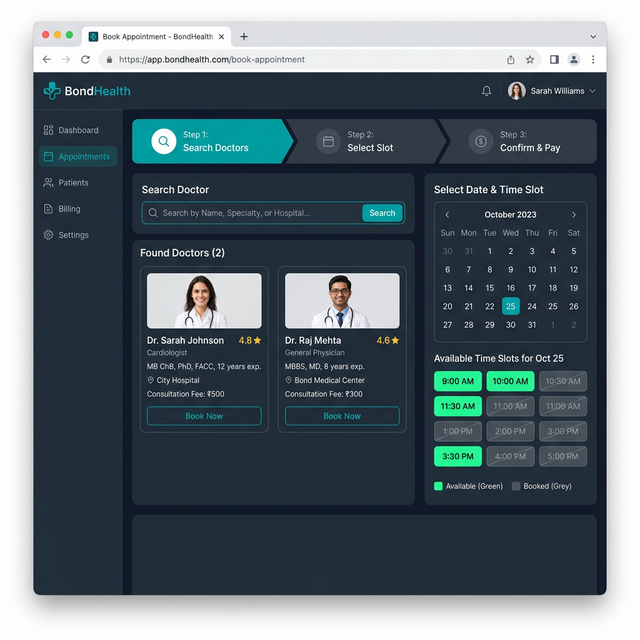
\includegraphics[width=0.85\textwidth]{images/chapter5/frontend_home.png}
\caption{Home Page / URL Input Screen}
\label{fig:frontend_home}
\end{figure}

The frontend is built with React using Vite as the build tool and Tailwind CSS for styling. Axios handles HTTP communication with the backend.

The home page provides a minimal interface containing a single URL input bar. The input supports deep-linking where the application reads the \texttt{?url=} query parameter and automatically triggers analysis.

\begin{figure}[h]
\centering
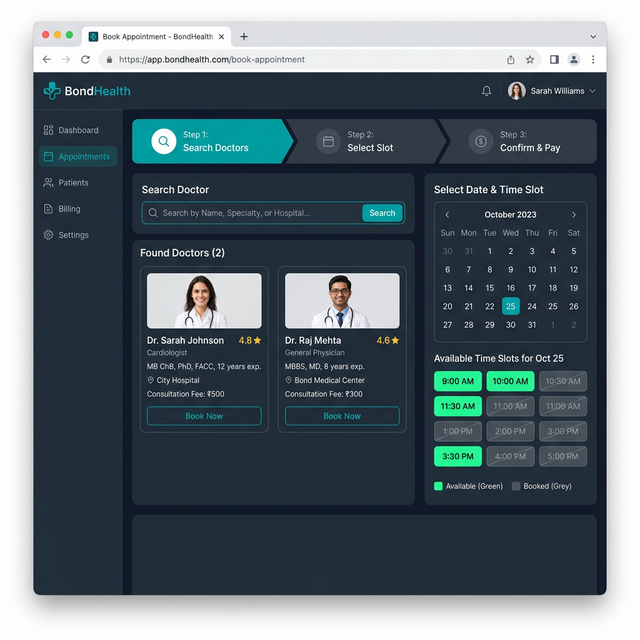
\includegraphics[width=0.85\textwidth]{images/chapter5/dashboard_score.png}
\caption{Analysis Results Dashboard — Score Gauge and Risk Label}
\label{fig:dashboard_score}
\end{figure}

Upon receiving backend results, the dashboard renders the composite risk score gauge, colour-coded risk label, recommendation string, and an ordered list of reasons.

\begin{figure}[h]
\centering
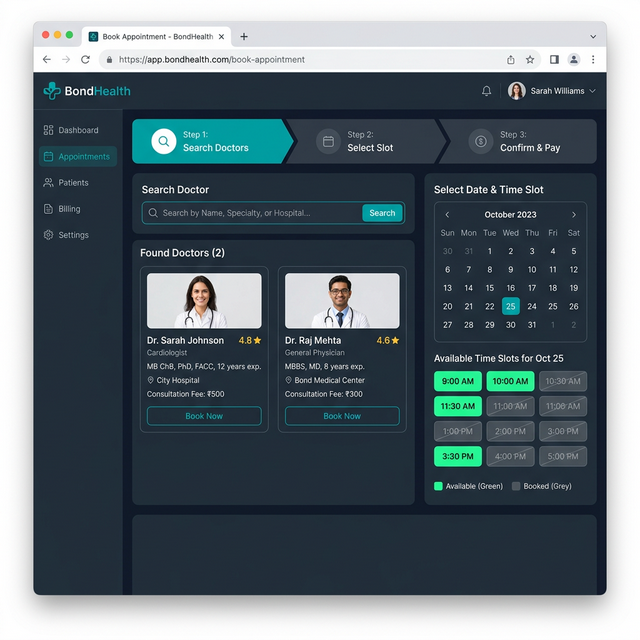
\includegraphics[width=0.8\textwidth]{images/chapter5/behavior_panel.png}
\caption{Behavior Panel — Redirects, External Requests, Suspicious Domains}
\label{fig:behavior_panel}
\end{figure}

The Behavior Panel displays redirect count, external requests, suspicious domains, redirect chains, and the final page title.

\begin{figure}[h]
\centering
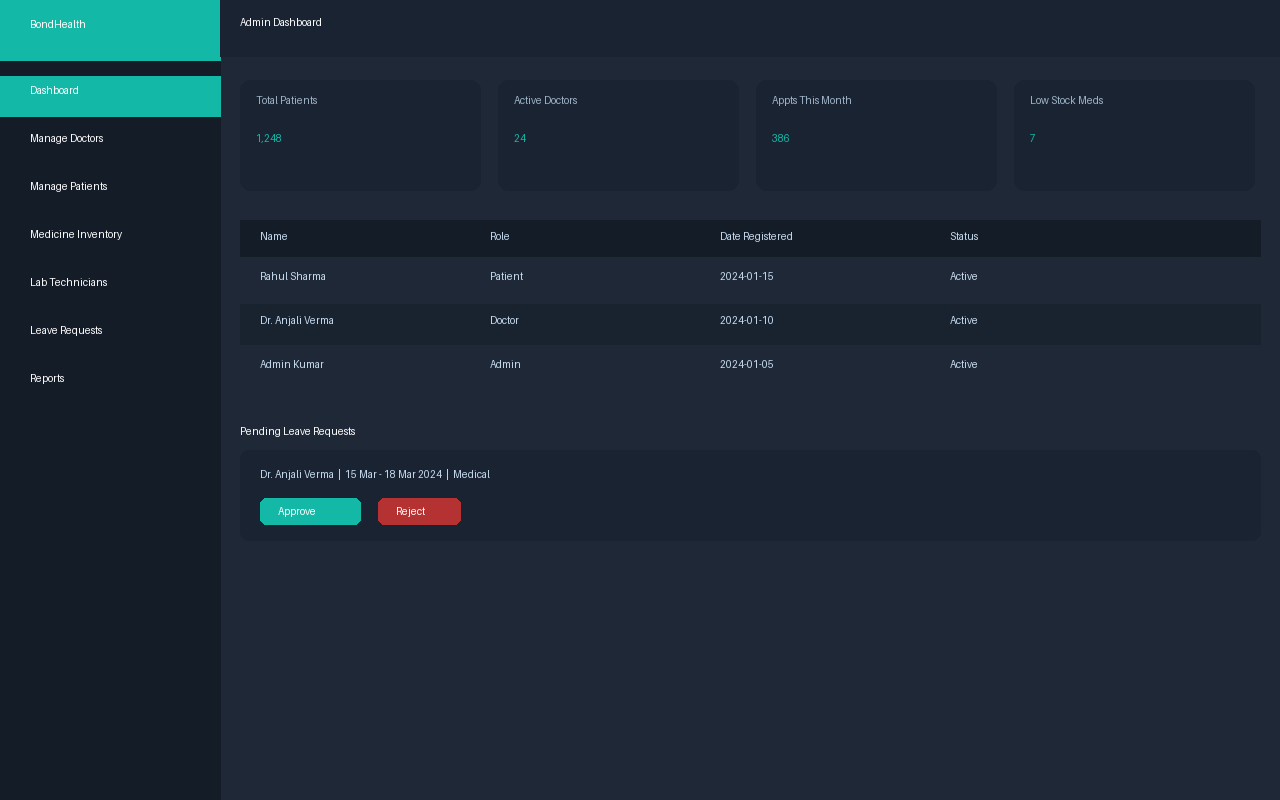
\includegraphics[width=0.8\textwidth]{images/chapter5/network_panel.png}
\caption{Network Panel — Domain Classification and Risk Level}
\label{fig:network_panel}
\end{figure}

The Network Panel presents the external domain count, safe infrastructure domains, suspicious domains, and overall network risk classification.

\begin{figure}[h]
\centering
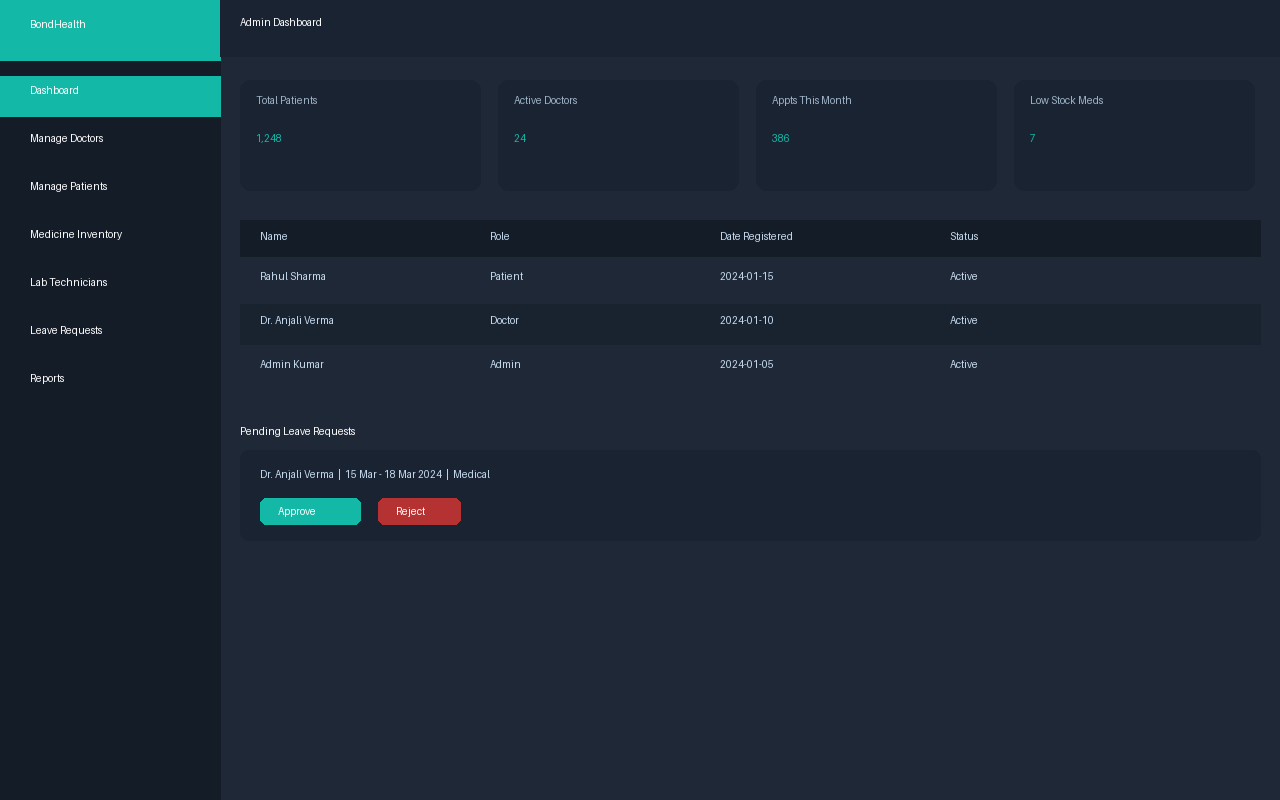
\includegraphics[width=0.8\textwidth]{images/chapter5/privacy_panel.png}
\caption{Privacy Panel — Exposure Bar, Fingerprinting Indicators, Cookie Counts}
\label{fig:privacy_panel}
\end{figure}

The Privacy Panel displays privacy grade, exposure bar, cookie counts, third-party scripts, and fingerprinting signals.

\begin{figure}[h]
\centering
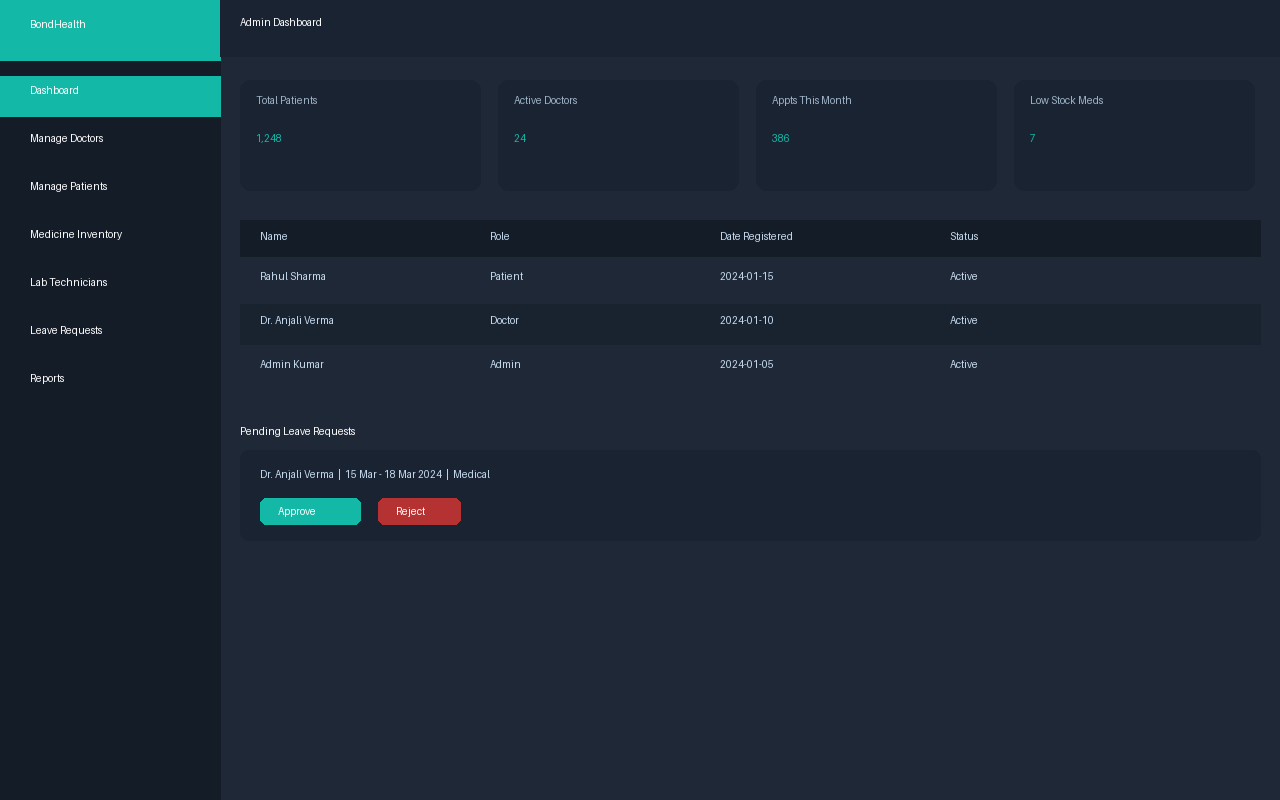
\includegraphics[width=0.8\textwidth]{images/chapter5/tracker_panel.png}
\caption{Tracker Panel — Named Tracker Detection}
\label{fig:tracker_panel}
\end{figure}

The Tracker Panel shows detected trackers including tracker name, matched domain, and HTML element type.

\subsection{Backend Development (Python / Flask)}

\begin{figure}[h]
\centering
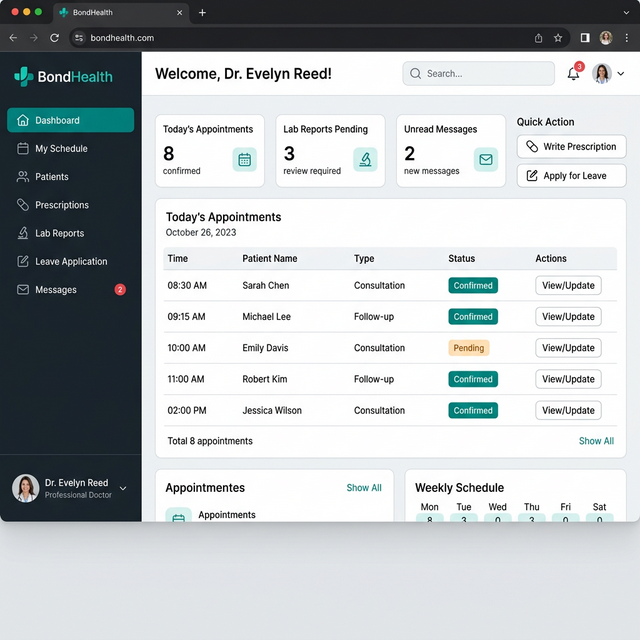
\includegraphics[width=0.8\textwidth]{images/chapter5/backend_routes.png}
\caption{app.py Route Structure and Parallel Execution}
\label{fig:backend_routes}
\end{figure}

The backend is implemented in Flask. The primary endpoint \texttt{POST /analyze} orchestrates the entire analysis pipeline.

Fast checks execute first, while slower network-dependent checks are executed concurrently using \texttt{ThreadPoolExecutor}. HTML content is fetched once and reused across multiple modules.

\begin{figure}[h]
\centering
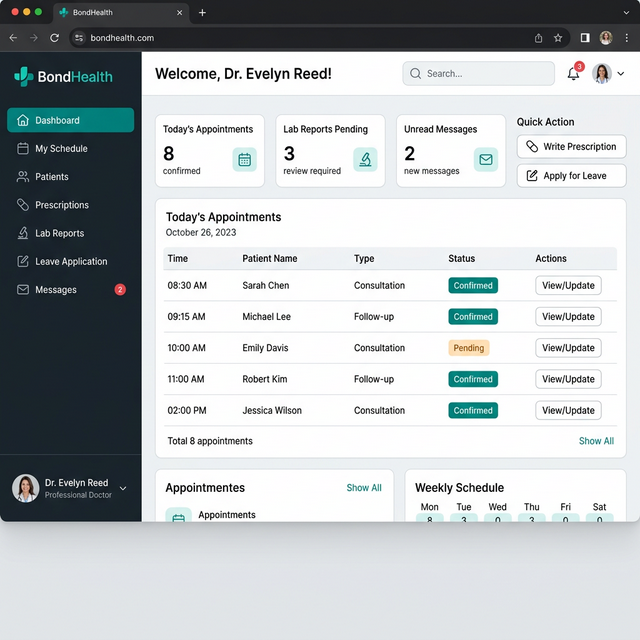
\includegraphics[width=0.75\textwidth]{images/chapter5/scoring_logic.png}
\caption{scorer.py Weighted Penalty Calculation}
\label{fig:scoring_logic}
\end{figure}

All module outputs are passed to \texttt{calculate\_risk\_score()} in \texttt{scorer.py}, which applies weighted penalties and compound signal amplification to produce the final score and label.

\subsection{Analysis Module Implementation}

\begin{figure}[h]
\centering
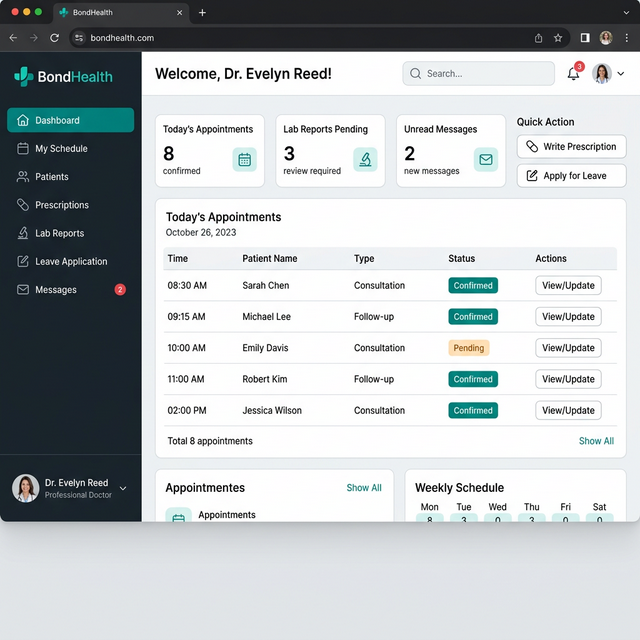
\includegraphics[width=0.75\textwidth]{images/chapter5/validator_pattern.png}
\caption{validator.py and pattern\_checker.py Implementation}
\label{fig:validator_pattern}
\end{figure}

The \texttt{validator.py} module normalises URLs and verifies HTTPS/TLS certificates before further analysis.

The \texttt{pattern\_checker.py} module performs lexical URL inspection to detect suspicious patterns.

\begin{figure}[h]
\centering
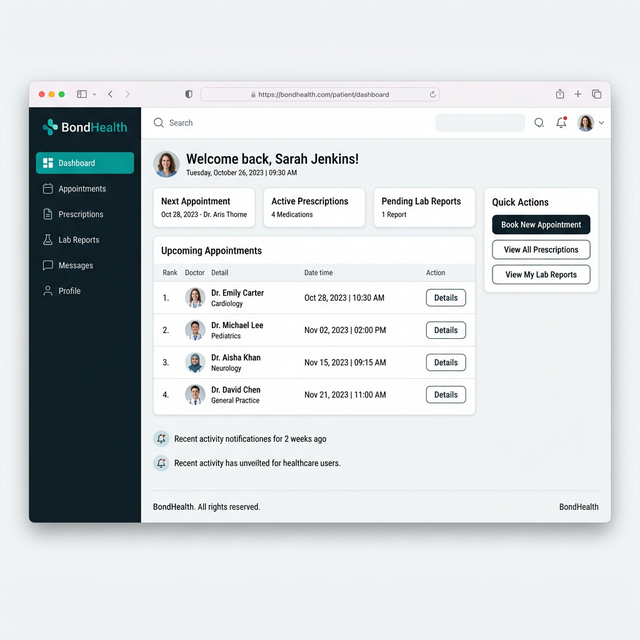
\includegraphics[width=0.75\textwidth]{images/chapter5/behavior_checker.png}
\caption{behavior\_checker.py Playwright Intercept Logic}
\label{fig:behavior_checker}
\end{figure}

The behavior module launches a headless Chromium browser using Playwright and intercepts redirect responses and network requests.

\begin{figure}[h]
\centering
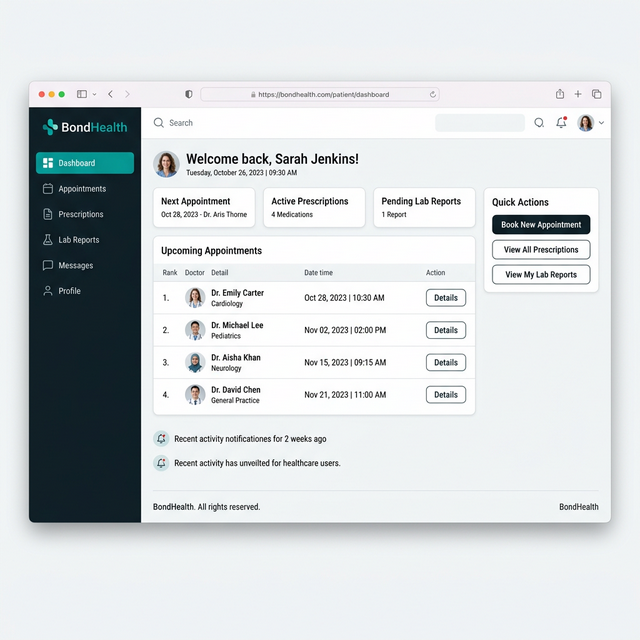
\includegraphics[width=0.75\textwidth]{images/chapter5/privacy_checker.png}
\caption{privacy\_checker.py Cookie and Fingerprinting Detection}
\label{fig:privacy_checker}
\end{figure}

The privacy module inspects cookies, tracking scripts, and browser fingerprinting techniques.

\subsection{Threat Intelligence Data Layer}

\begin{figure}[h]
\centering
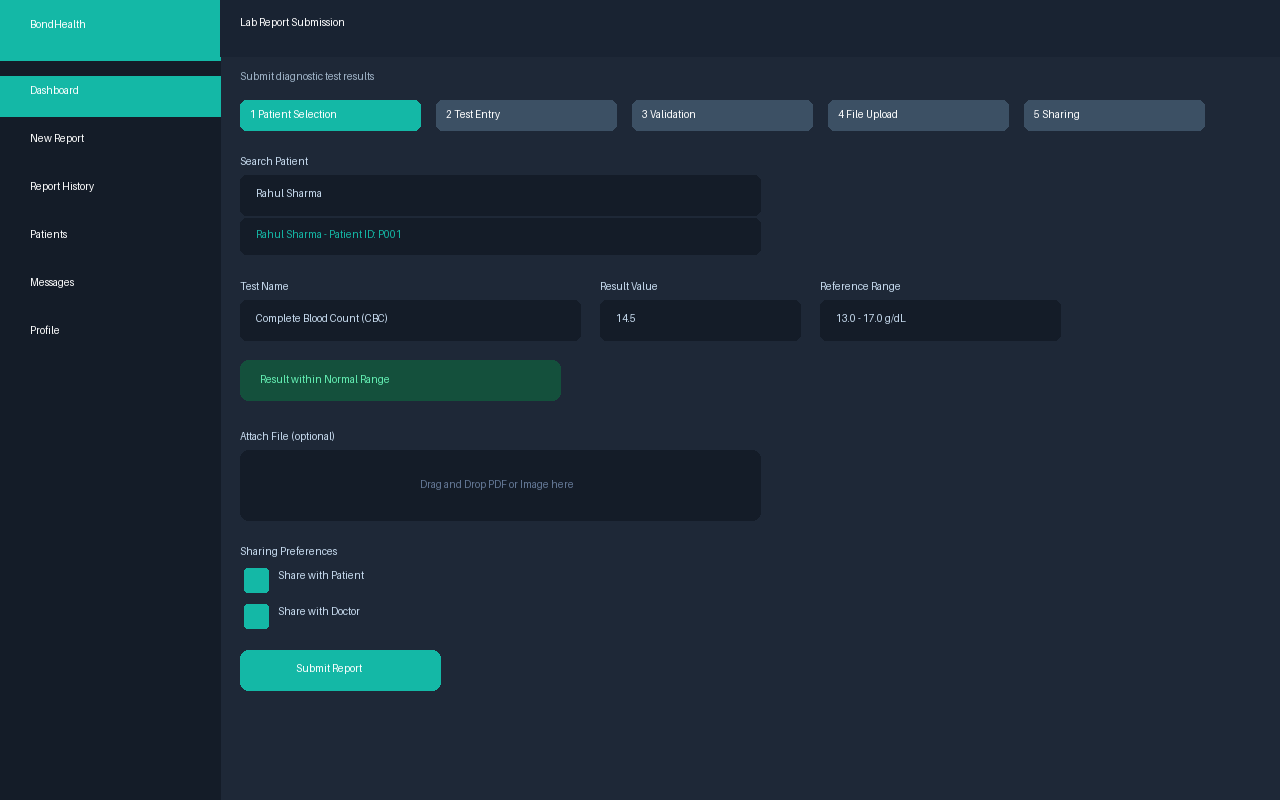
\includegraphics[width=0.75\textwidth]{images/chapter5/urlhaus_updater.png}
\caption{URLhaus Feed Download and CSV Extraction}
\label{fig:urlhaus_updater}
\end{figure}

The threat intelligence layer downloads the URLhaus blacklist feed and loads it into memory for fast domain lookups.

\subsection{Browser Extension Implementation}

\begin{figure}[h]
\centering
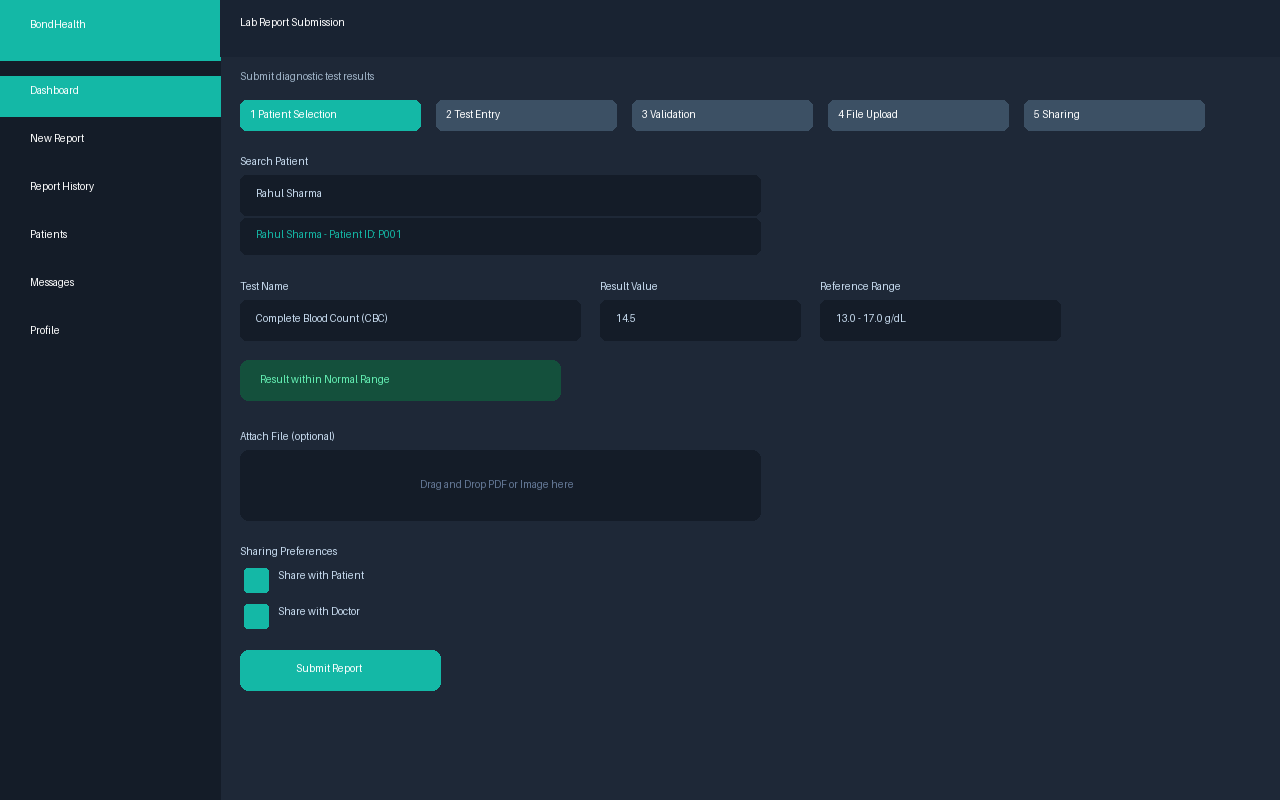
\includegraphics[width=0.75\textwidth]{images/chapter5/extension_overview.png}
\caption{Browser Extension Popup — Overview Tab}
\label{fig:extension_overview}
\end{figure}

The Chrome extension uses Manifest V3 and communicates with the Flask backend to analyze the active tab URL.

\begin{figure}[h]
\centering
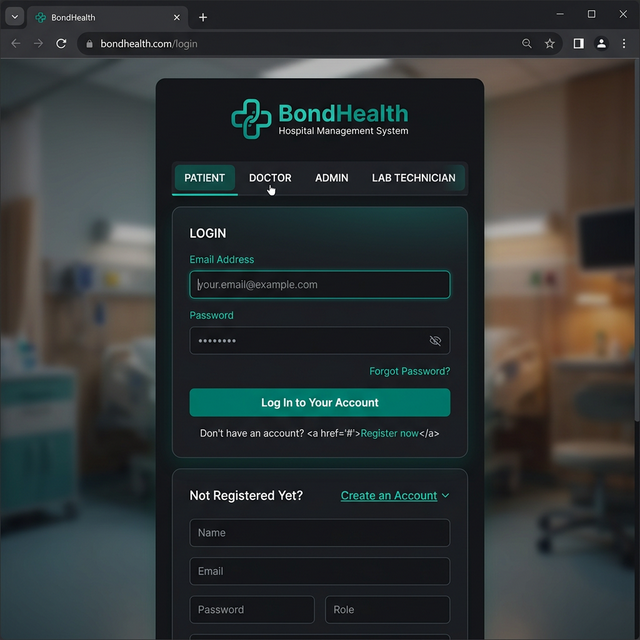
\includegraphics[width=0.75\textwidth]{images/chapter5/extension_privacy.png}
\caption{Browser Extension Popup — Behavior and Privacy Tabs}
\label{fig:extension_privacy}
\end{figure}

The popup UI displays the score arc, risk label, status indicators, and detailed analysis tabs.

\subsection{Fast Mode and Caching}

\begin{figure}[h]
\centering
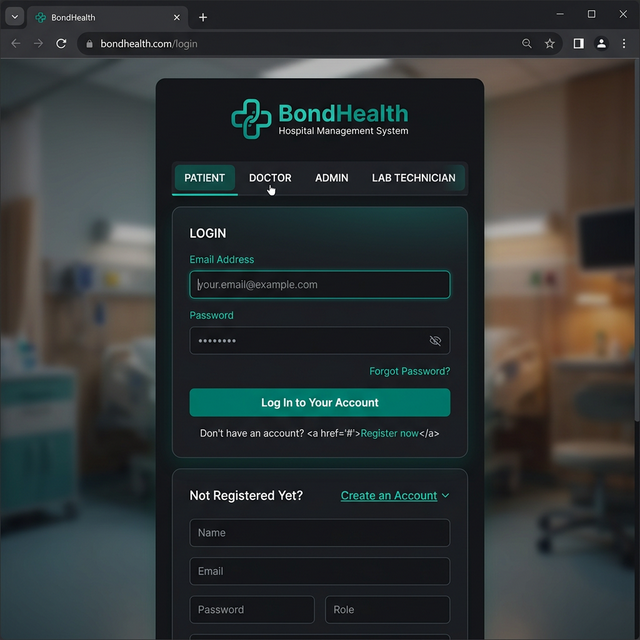
\includegraphics[width=0.75\textwidth]{images/chapter5/cache_fastmode.png}
\caption{Fast Mode and Result Cache Logic in app.py}
\label{fig:cache_fastmode}
\end{figure}

Fast Mode bypasses Playwright runtime analysis to reduce total execution time. A result cache stores recently analyzed URLs for 30 minutes to prevent redundant scans.